\documentclass[tikz]{standalone}

\usetikzlibrary{decorations.pathmorphing,patterns}
\begin{document}
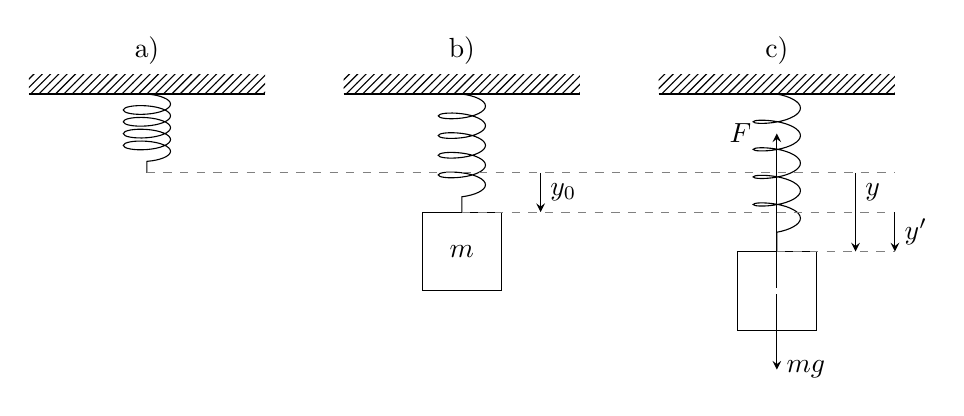
\begin{tikzpicture}
		%Roofs
		\fill [pattern = north east lines] (0,0) rectangle (3,0.25) node[above] at (1.5, 0.25) {a)};
		\draw[thick] (0,0) -- (3,0);
		
		\fill [pattern = north east lines] (4,0) rectangle (7,0.25) node[above] at (5.5, 0.25) {b)};
		\draw[thick] (4,0) -- (7,0);
		
		\fill [pattern = north east lines] (8,0) rectangle (11,0.25) node[above] at (9.5, 0.25) {c)};
		\draw[thick] (8,0) -- (11,0);
		
		%Springs
		\draw[decoration={aspect=0.3, segment length=1.5mm, amplitude=3mm,coil},decorate] (1.5,0) -- (1.5,-1); 
		
		\draw[decoration={aspect=0.3, segment length=2.5mm, amplitude=3mm,coil},decorate] (5.5,0) -- (5.5,-1.5); 
		
		\draw[decoration={aspect=0.3, segment length=3.5mm, amplitude=3mm,coil},decorate] (9.5,0) -- (9.5,-2); 
		
		%Boxes
		\draw (5,-1.5) rectangle (6,-2.5);
		\node at (5.5,-2) {$m$};
		
		\draw (9,-2) rectangle (10,-3);
		%\node at (9.5,-2.5) {$m$};
		
		%Horizontal lines
		\draw[gray, dashed] (1.5,-1) -- (11,-1);
		\draw[gray, dashed] (5.5,-1.5) -- (11,-1.5);
		\draw[gray, dashed] (9.5,-2) -- (11,-2);
		
		%Vertical displacements
		\draw[-stealth] (6.5,-1) -- (6.5,-1.5);
		\node[right] at (6.5, -1.25) {$y_0$};
		
		\draw[-stealth] (10.5,-1) -- (10.5,-2);
		\node[right] at (10.5, -1.25) {$y$};
		
		\draw[-stealth] (11, -1.5) -- (11, -2);
		\node[right] at (11, -1.75) {$y'$};
		
		%Forces
		\draw[-stealth] (9.5,-2.54) -- (9.5, -3.5);
		\node[right] at (9.5, -3.5) {$mg$};
		
		\draw[-stealth] (9.5, -2.46) -- (9.5, -0.5);
		\node[left] at (9.3, -0.5) {$F$};
	\end{tikzpicture}
\end{document}